\documentclass[UTF8]{ctexart}

\usepackage{amsfonts} % 数学字体支持
\usepackage{amsmath} % 数学啊啊支持
\usepackage{makeidx} % 参考文献编号支持?
\usepackage{graphicx} % 图片支持

\graphicspath{{figure/}}

\title{工业数据统计分析与应用课程报告\\——用于线性回归的面部识别算法}
\author{刘永峰\thanks{自动化学院}}
\date{\today}

\makeindex
\bibliographystyle{...}

\begin{document}

\maketitle % 标题页
\begin{abstract}
    本文旨在对用于面部识别的线性回归分类算法(Linear Regression Classification)进行重现并呈现实验结果。该线性回归分类算法将待识别图像表示为根据类进行划分的一组图像的线性组合,它使用最小二乘法对前述问题的系数向量进行求解并生成预测器,并根据不同类预测器生成的预测结果与待识别图片的距离来判断其所属类别。本文将该算法用于AT\&T面部图像数据库并进行了有关参数的调试。另外还对跟随LRC算法同时提出的用于处理人脸图像中连续覆盖物的模块化LRC(Modular LRC)进行了描述,但由于时间原因,并未进行重现。\\
    \textbf{关键词}:面部识别,线性回归算法
\end{abstract}
\section{引入}\label{sec-1}
面部识别算法的效果依赖于多种有关工具的设计和选择。首先,一个\(a \times b\)维的灰度面部图像可以被表示为在原始图像空间(image space)的\(ab\)维的向量。但是如果直接处理类似数据量的原始数据会导致严重的维数灾难,以至于在一些情况下完全无法完成处理。所以研究者希望在特征提取阶段将原始数据在保证能够对面部进行区分的条件下降维到面部空间(face space)。在这种目标的驱动下产生并应用了一系列的特征提取方法,如主成分分析(Principle Component Analysis, PCA)、线性判别(Linear Discriminant Analysis, LDA)和独立成分分析(Independent Component Analysis, ICA)等等。前述方法大体上可以分为两种类型:重构型(reconstructive)和判别型(discriminative)。重构型方法对于受污染像素的处理更为有效,而判别型的方法则相对更为适合原始数据较为干净的情况。除了以上这些传统的方法之外,研究者发现似乎诸如下采样(downsampling)、随机投影等等一些非“正统”的方法方法在实际应用上也同样有效。于是,确定特征空间维度和分类器的设计就成了影响算法效果的重中之重。\par
本文基于Imran Naseem等人发表于2010年的文章Lnear Regression for Face Recognition中的LRC算法进行重现。在该文中,作者提出了简单有效LRC算法用于进行面部识别。该算法基于这样一条准则,即\textit{某种类别的所有样本都会落在同一个线性子空间内},从而使用线性回归对面部识别问题进行处理。其中反映待分类图像与类模型之间关系的参数向量由最小二乘估计给出。最终,根据每类对待分类模型预测的准确度来确定图像所属类别。该方法可被视作一种最近邻子空间(Nearest Subspace, NS)方法。\par
LCR算法所基于的最重要的工作在文献【】中进行了描述。其在训练阶段使用所有的下采样后的图像用于生成字典矩阵(dictionary matrix),然后将待分类图像表示为各个字典矩阵中向量的线性组合,从而构成了一个病态逆问题(ill-conditioned inverse problem)。该问题中所存在系数向量稀疏性问题(sparsity of the vector of coefficients)可以利用线性范数极小化(\(l_1\)-norm minimization)方法来求解。文献【】中,局部线性回归(Locally Linear Regression, LLR)方法被用于处理朝向不同的面部图像。该文献阐述了面部侧面图像和正面图像的近似线性映射关系并给出了将该问题的求解化为一个累进解的预测问题的方法。对于变化较为严重的摆姿,则对不同朝向的图像进行采样,得到很多交叠的局部段落,从而可以使用这些小的段落,对正面人像进行分类。LLR算法在校准较为粗略的面部图像识别之中获得了一些优异的表现。文献【】中提出了一种两阶段的方法,该方法在特征提取阶段将小波分解(wavelet decomposition)和判别分析(discriminant analysis)结合,提取的特征用于构建特征平面和特征空间。最终将待分类图像投影到子空间之中并根据最小距离来判断所属类别。而LCR算法则采用更为基础的方法得到了较之前两例基准算法更为优异的表现。\par
进一步的,LCR算法还针对严重的连续遮挡物提出了一种图像的模块化表示方法,并给出了模块化的LCR算法用于求解该类图像的识别问题。该方法将存在连续遮挡的图像进行分割,并对每个分割进行判别,然后使用名为基于距离的证据融合(Distance-based Evidence Fusion, DEF)算法对最终结果进行预测。分割方式的好坏则是通过对中间决策(即不同分块的类型判别结果)构成的距离矩阵进行评估来进行判断。该类方法的优势有:第一,通过距离矩阵的评估和证据融合避免了遮挡部分参与并影响判断结果;第二,证据融合使最终判断结果优于最优的独立分块的判断结果。\par
以下内容将分为几个部分进行阐述:第二部分介绍了LRC和模块化LRC算法,第三部分将对实验结果进行大致描述,第四部分是总结与展望的内容。
\section{用于面部识别的线性回归算法}\label{sec-2}
以下内容将对面部识别的LRC算法和用于处理连续遮挡的图像的模块化处理方法分别进行阐述。
\subsection{线性回归分类器}
该方法简而言之就是使用多组分类后的含标签图像向量构成预测器,并估计每组图像向量集对目标图像向量的\textbf{线性组合},估计最为精确的那一类——即线性组合后得到的响应向量距离目标图像向量最近者即为目标图像所属的类型。具体流程如下:\par
设有\(N\)个互相区别的类,其中第\(i\)类中包含\(p_i\)个训练图像,\(i=1,2,...,N\)。每个\(a \times b\)维的灰度训练图像可以被表示为\({\stackrel{(m)}{u_i}} \in {\mathbb{R}^{q \times 1}}, i = 1,2,\dots,N\)且\(m = 1,2,\dots,p_i\)。其中每个训练图像均被下采样到\(c \times d\)维,并且通过列连接(column concatenation)转换为列向量,即\({\stackrel{(m)}{u_i}} \in {\mathbb{R}^{q \times 1}} \rightarrow {\mathbf{w}_i} \in \mathbb{R}^{q \times 1}\),其中【】。每个图像向量均进行归一化令灰度最大值像素值为1。基于同一个类型的样本均落在同一个线性子空间中的准则,通过将同一类的\(q\)维图像向量进行堆积,可以得出如下的类型划分模型,
\begin{equation}
    {\mathbf{X}_i = [\stackrel{(1)}{\mathbf{w}_i} \quad \stackrel{(2)}{\mathbf{w}_i} \dots \stackrel{(p_i)}{\mathbf{w}_i}] \in \mathbb{R}^{q \times p_i}},\quad i=1,2,\dots,N
\end{equation}
其中每个向量构成的子空间【】也是【】的列空间。即每个类型\(i\)都可以被表示为子空间\(\mathbf{X}_i\),【】也被称作类型\(i\)的回归器(regressor)或者预测器(predictor)。如果设\(z\)是一个无标签灰度图像,则我们的问题就可以表示为求\(z\)所从属的类别\(i\),此处\(i=1,2,...,N\)。我们将\(z\)也做与训练图像相同的转换,即进行归一化和列连接将之转换为图像向量\(\mathbf{y}\),即\(\mathbf{y}\in\mathbb{R}^{q \times 1}\)。如果\(\mathbf{y}\)属于第\(i\)类,则它可以表示为相同类别的训练图像的线性组合(也就是说它与该组训练图像会落在相同的子空间内),即,
\begin{equation}\label{eq-2} % 注意交叉引用标签命名,不能直接使用eq2好像
    \mathbf{y}=\mathbf{X}_i\beta_i,\quad i=1,2,\ldots,N,
\end{equation}
% \eqref用于公式的交叉引用
其中\(\beta_i\in\mathbb{R}^{p_i \times 1}\)是参数向量,已知\(q \ge p_i\),公式\eqref{eq-2}中的系统是\textbf{良态}(well conditioned)的,从而可以使用最小二乘估计来估计\(\beta\),公式如下:
\begin{equation}\label{eq-3}
    \hat{\beta}={(\mathbf{X}^T_i\mathbf{X}_i)^{-1}\mathbf{X}^T_i\mathbf{y}}
\end{equation}
\par
从而得到的参数向量\(\beta\)以及预测器\(\mathbf{X}_i\)可以用来预测每个类的响应向量(response vector),公式及相关变换如下:
\begin{equation}\label{eq-4}
    \begin{split}
        & \hat{\mathbf{y}}_i={\mathbf{X}_i\hat{\beta}_i}\\
        & \hat{\mathbf{y}}_i={\mathbf{X}_i{(\mathbf{X}^T_i\mathbf{X}_i)}^{-1}{\mathbf{X}^T_i\mathbf{y}}}\\
        & {\hat{\mathbf{y}}_i}={\mathbf{H}_i\mathbf{y}},
    \end{split}
\end{equation}
式中预测向量(响应向量)\(\hat{\mathbf{y}}\in\mathbb{R}^{q \times 1}\)是\(\mathbf{y}\)在第\(i\)个子空间中的投影。实际上也就是说\(\hat{y}_i\)是在子空间\(i\)中相距观察向量(observation vector)\(\mathbf{y}\)欧氏距离最近的向量。而其中将\(\hat{\mathbf{y}}\)转换为\(\mathbf{y}\)的矩阵\(H\)被称作帽子矩阵(hat matrix)。有了\(\hat{\mathbf{y}}_i\)和\(\mathbf{y}\),我们就可以计算\(\mathbf{y}\)和不同类的估计向量\({\hat{\mathbf{y}}}_i\)之间的欧氏距离:
\begin{equation}\label{eq-5}
    d_i(\mathbf{y})={\|\mathbf{y}-{\hat{\mathbf{y}}}_i\|}_2,\quad i=1,2,\dots,N
\end{equation}
得到了两者的欧氏距离之后,其中与\(\mathbf{y}\)相距欧氏距离最小的\(\hat{\mathbf{y}}_i\)所属的类别\(i\)就是\(\mathbf{y}\)所属的类别,即
\begin{equation}
    \underbrace{\min}_i d_i(\mathbf{y}),\quad i=1,2,\dots,N.
\end{equation}

\subsection{线性回归分类器中的图像模块化方法}
\texttt{作者在文献【】中还提出了一种用于处理连续遮蔽的图像模块化工具,由于使用的带有遮蔽的面部图像数据库在文中需要进行手动对齐,基于工作量和报告上交时间考虑并未进行重现,但在此也一并介绍之。}\par
局部遮挡的面部识别问题可以用图像模块化方法来处理,因为局部连续遮挡物虽然遮挡范围可能有所不同,但是由于其是连续的,所以只是污染了一部分像素,所以采取特定方法将之区分即可。而分块的图片表示方法可以有效地处理这类问题。文献【】中的分块处理方法则是将原始图像分为几个部分,每个部分都进行独立的线性回归,然后将所有的部分得到的证据进行融合得出最后的分类结果。当然最简单的决策融合方法可能就是多数表决(majority voting)【】了,但该方法将污染部分和未污染部分等效看待,可能会引发问题。试想如果四块图像三块都是被污染的部分,那么如果进行多数表决那么无论无污染部分和原始图像匹配有多么显著,最终结果仍然是被污染部分的决策结果占据优势,而毫无疑问,被污染部分在决策过程中不应当拥有这样的权重。另问题更为复杂的是污染分布并不是先验的,可能分布在非面部区域,也可能分布在面部区域。据此,有人提出了复杂的污染像素剔除算法【】。\par
而对于这种问题,参照文献【】中给出的方法则较为简单。该方法基于距离分类,自然而隐式地降低了被污染子图像的决策权重,从而显著提高了分类精度。该方法被称为“基于距离的证据融合(Distance-based Evidence Fusion)”,具体方法如下:
假设每个训练图像均被划分为\(M\)个部分,每个部分用\(v_n,\ n=1,2,\dots,M\)表示。其中全部\(p_i\)个训练图像的第\(n\)个子图像均按照章节\ref{sec-2}所述进行下采样和列连接处理并最终构成分类-分区子空间\(\mathbf{U}^{n}_i\):
\begin{equation}
    \mathbf{U}^{(n)}_i=[\stackrel{(1)^{(n)}}{\mathbf{w}_i}\stackrel{(2)^{(n)}}{\mathbf{w}_i}\ldots\ldots\stackrel{(3)^{(n)}}{\mathbf{w}_i}],\quad i=1,2,\dots,N.
\end{equation}
每个分类均可以被表示为\(M\)个子空间,于是我们得到了具有\(M\times N\)个子空间的分类模型。对于待分类图像我们也划分为\(M\)块并对每块进行列连接处理转化为图片向量\(\mathbf{y}^{(n)},n=1,2,\dots,M\)。已知\(i\)为该待分类图像所属的类别,那么\(\mathbf{y}^{(n)}\)就应当位于分类器\(\mathbf{U}^{(n)}_i\)的第\(n\)个子空间,即应当满足
\begin{equation}
    \mathbf{y}^{(n)}=\mathbf{U}^{(n)}_i\beta^{(n)}_i
\end{equation}
于是乎类似于LRC的逻辑,参数向量和预测图像向量可以由下式计算得出:
\begin{align}
    \hat{\beta}^{(n)}_i&={[(\mathbf{U}^{(n)}_i)^T\mathbf{U}^{(n)}_i]}^{-1}(\mathbf{U}^{(n)}_i)^T\mathbf{y}^{(n)},\\
    \hat{\mathbf{y}}^{(n)}_i&=\mathbf{U}^{(n)}_i{\hat{\beta}}^{(n)}_i;\quad i=1,2,\dots,N.
\end{align}
\par
同时估计图像向量和原始图像向量的距离也由类似LRC的逻辑给出:
\begin{equation}
    d_i(\mathbf{y}^{(n)})=\|\mathbf{y}^{(n)}-\mathbf{y}^{(n)}_i\|_2;\quad i=1,2,\dots,N.
\end{equation}
\par
现在对于分块\(n\)我们可以进行其所属分类的决策了,该决策被称为中间决策(intermediate decision),表示为\(j^{(n)}\),该决策类似前文,由最小距离给出,而我们暂时需要的是该决策所对应的距离:
\begin{equation}
    d^{j^{(n)}}=\underbrace{\min}_i d_i(\mathbf{y}^{(n)})\quad i=1,2,\dots,N
\end{equation}
至此我们有\(M\)个子图像决策距离了,融合决策的步骤也很简单,就是直接选取这\(M\)个中间决策中距离最小的那个所对应的决策,即为最终决策:
\begin{equation}
    Decision=\arg{\underbrace{\min}_j}d^{j^{(n)}}\quad n=1,2,\dots,M.
\end{equation}
\section{实验结果}\label{sec-3}
算法重现之后对该算法进行了一些实验,对比了其中一些具体设置所能导致的差异,使用的测试数据为AT&T人脸数据库。
\begin{figure}[h]
    \centering
    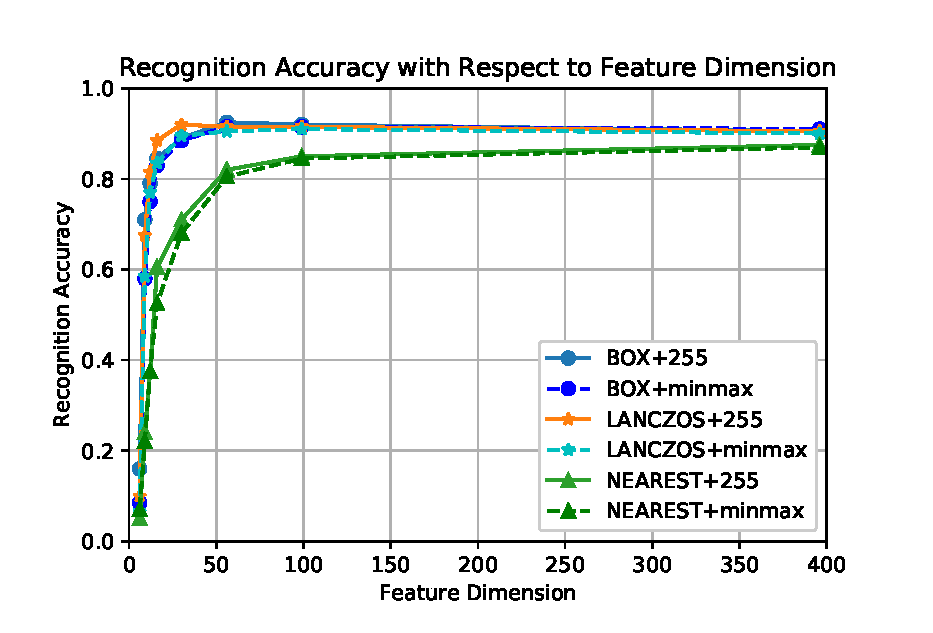
\includegraphics[scale = 0.6]{RA_Method.eps}
    \caption{使用不同类型归一化方法的识别精度差异}\label{fig-1}
\end{figure}
\begin{figure}[h]
    \centering
    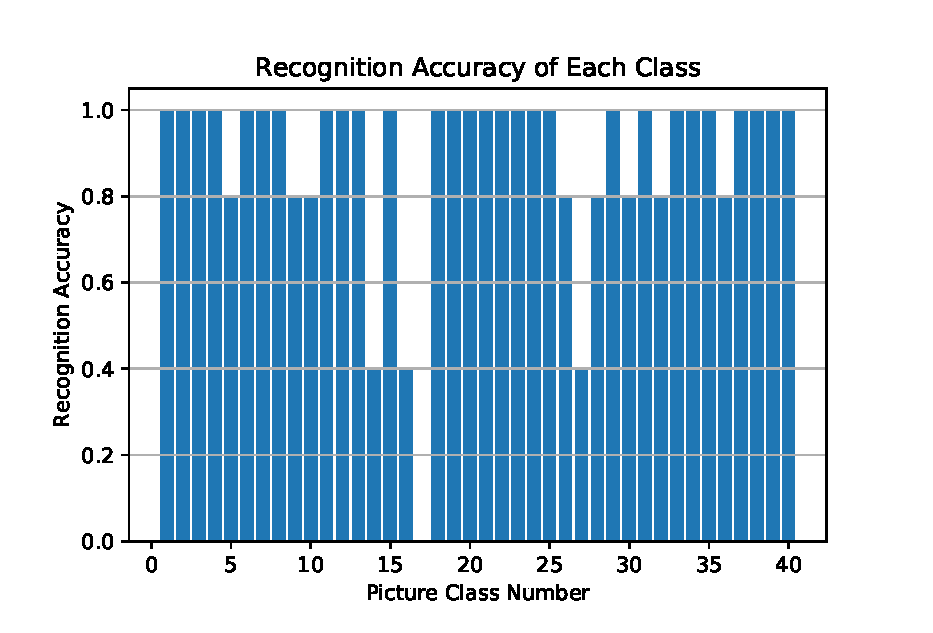
\includegraphics[scale = 0.6]{RA_Class.eps}
    \caption{啥玩意}\label{fig-2}
\end{figure}

\section{总结与展望}\label{sec-4}

中文文档类测试。你需要将所有源文件保存为UTF-8 编码。
你可以使用XeLaTeX、LuaLaTeX 或upLaTeX 编译,也可以使用(pdf)LaTeX 编译。
推荐使用XeLaTeX 或LuaLaTeX 编译。
\appendix
\include{code} % 附录A appendixA.tex

\bibliography{...} % 利用BibTeX 工具生成参考文献
\printindex % 利用makeindex 工具生成索引
\end{document}